%\documentclass[a4paper, 11pt]{article}
%\usepackage[cm]{fullpage}
%\usepackage[english]{babel}
%\usepackage[latin1]{inputenc}
%\usepackage[T1]{fontenc}
%\usepackage{color}
%\usepackage{ulem}
%\usepackage{fancyvrb}
%\usepackage{amsmath}
%\usepackage{amsfonts}
%\usepackage{graphicx} 
%\usepackage{xcolor}
%\usepackage{listings}
%\usepackage{textcomp}
%
%\usepackage{tikz}
%\usepackage{circuitikz}
%\usepackage{pgfplots}
%\usepackage{graphicx}
%\usetikzlibrary{calc,through,backgrounds}
%\usetikzlibrary{decorations.markings,decorations.pathmorphing,decorations.pathreplacing}
%\usetikzlibrary{arrows,shapes,positioning}
 %\tikzstyle arrowstyle=[scale=1]
 %\tikzstyle directed=[postaction={decorate,decoration={markings,
    %mark=at position .5 with {\arrow[arrowstyle]{stealth}}}}]
 %\tikzstyle reverse directed=[postaction={decorate,decoration={markings, 
   %mark=at position .5 with {\arrowreversed[arrowstyle]{stealth};}}}]
%\usepackage{rotating}
%\usepackage{multirow}
%\pgfplotsset{compat=1.10}
%
%\newcounter{examplecounter}
%\newenvironment{example}{\begin{quote}
    %\refstepcounter{examplecounter}
  %\textbf{Example \arabic{examplecounter}}
  %\quad}{\end{quote}}
%
%\newcounter{lemmacounter}
%\newenvironment{lemma}{\begin{quote}
    %\refstepcounter{lemmacounter}
  %\textbf{Lemma \arabic{lemmacounter}}
  %\quad}{\end{quote}}
%
%\newcounter{propcounter}
%\newenvironment{proposition}{\begin{quote}
    %\refstepcounter{propcounter}
  %\textbf{Proposition \arabic{propcounter}}
  %\quad}{\end{quote}}
%
%\title{LINMA2471 - Optimization\\
%Cours 5}
%\author{S. \textsc{Cheng}, Q. \textsc{Le}, F. \textsc{Delcourt}}
%\date{\today}
 %
 %
%\begin{document} 
%\maketitle


We've been investing in convex models and trying to find the best formulation of optimization problems. We now explore different methods that allow us to solve those problems and study their properties. In this part we focus on first order methods. Second order methods will be discussed further.

\section{Gradient Method}

A main example of first order methods is the Gradient Method also known as the Steepest Descent Method. Many practical problems have constraints but let's consider for the moment that we have none.  
 
Problem:  $\underset{x  \in \mathbb{R}^n}{\text{min }} \: f(x) $
 
\begin{lstlisting}[mathescape,caption=Gradient Algorithm]
Given $x_0$, $k=0$
Repeat
$x_{k+1} = x_k - \underbrace{h_k}_{\in \mathbb{R}} \underbrace{\nabla f(x_k)}_{\in \mathbb{R}^n}$
$k \leftarrow k+1$
\end{lstlisting}

$h_k$ is called the step length and $-\nabla f(x_k)$ is called the direction.


\section{Step length selection}

\subsection{ $h_k$ that minimize $f(x_k - h_k \nabla f(x_k))$} 

We have to solve for $h_k$ at each step. Even if we only minimize one variable, it's still an iterative method and does not give directly $h_k$. 

\subsection{$h_k = \alpha$}

\begin{example}\begin{leftbar}
Let's consider $x^2$ and see what happens when we change $h_k$

\framebox[1.5cm][c]{$h_k = 2$} $\quad \forall k$ \\
Set $x_0$ \\
$x_1 = x_0 - 2(2x_0) = -3x_0$\\
$x_2 = -3x_0 - 2(-6x_0) = 9 x_0$\\
Instead of going to zero we go to $-3x_0$ or $9x_0$. Our step is clearly too large. This is called DIVERGING.

\framebox[1.5cm][c]{$h_k = 1$} $\quad \forall k$ \\
$x_1 = x_0 - 2x_0 = -x_0$\\
$x_2 = = -x_0 - (-2x_0) = x_0$ \\
This time, we are still too large and this is called CYCLING. 

\framebox[1.5cm][c]{$h_k = \frac{1}{2}$} $\quad \forall k$ \\
$x_1 = x_0 - \frac{1}{2}(2x_0)$ = 0 \\
We have a FINITE CONVERGENCE. 

\framebox[1.5cm][c]{$h_k = \frac{1}{3}$} $\quad \forall k$ \\
$x_1 = x_0 - \frac{1}{3}(2x_0) = \frac{1}{3}x_0$\\
$x_2 = \frac{1}{3}x_0 - \frac{1}{3}(2\frac{1}{3}x_0) = \frac{1}{9}x_0$\\
$\vdots$\\
$x_k = \frac{1}{3^k}x_0$ \\

We get closer to $x_0$. 

\end{leftbar}\end{example}

The simple gradient method is subjected to poor step length selection. However it still good to use a constant step length. We'll explicitly and numerically compute some value of $\alpha$ which guarantee a good behavior. 

\subsection{$h_k$ satisfies some "dynamic" conditions (e.g. Wolfe condition)}

In order to know what is the best step length, we need to know the function. We focus only on functions that are $C_L^{1,1}$, which means that $f \in C^1$ and $\nabla f$ is Lipschitz with constant L. The Lipschitz condition is:
$$\| \nabla f(x) - \nabla f(y) \| \leq L \| x-y \|$$
In order words, if we take 2 points, their gradient can't be too different.\\

Mathematically, we can define: 

\begin{definition}
Given $L>0$, we say $f : D \subseteq \mathbb{R}^n \to \mathbb{R}$ has \emph{$L$-Lipschitz gradient} if and only if $f \in C^1(D)$ and
\begin{equation*}
\vnorm{\nabla f(x) - \nabla f(y)} \le L \vnorm{x-y}
\end{equation*}
for all $x,y \in D$. We denote $C_L^{1,1}(D)$ the set of such functions. We also define
\begin{equation*}
F_L^{1,1}(D) = \{ f \in C_L^{1,1}(D) \mid f \text{ is convex}\} .
\end{equation*}
\end{definition}

Given $f \in C^1$, we also denote $T^1_y(x) = f(y) + \nabla f(y)^T (x-y)$ the first-order Taylor expansion of $f$ around $y$ evaluated at point $x$.


\begin{example}\begin{leftbar}
Function that are Lipschitz with L=0? Linear function are $C_0^{1,1}$
\end{leftbar}\end{example}

\begin{example}\begin{leftbar}
Standard quadratic function $x \rightarrow x^T Q x $  with no convexity assumption for now. The Lipschitz condition can be expressed as: 
$$ \| 2Qx - 2Qy \| \leq L \| x-y \|  \quad \forall x,y$$
$$ 2 \| Q (x -y)  \| \leq L \| x-y \| \quad \forall x,y$$
If $Q=Id$, it's clear that $L = 2$.  When it comes to matrix like Q, we will use the spectral norm. From the matrix theory, we  know that:
$$ \| Qv \|_2 \leq \underbrace{\| Q\| _2}_{max \vert \lambda_i (Q) \vert} \| v \|_2$$

One can hence choose $$L=2 \| Q \|_2 $$

For more complicated function, we can try to bound the value of L  and use  its estimate. 
\end{leftbar}\end{example}

As we can see, it's very easy to compute the constant for a quadratic function. But what can we do in a more  general case?\\

\begin{property} 
When f  $ \in C^2$ the Lipschitz constant is given by $ L=\underset{x}{\text{max }} \| \nabla^2 f(x) \|$ .
\label{5:prop1}
\end{property}
This result is very useful for one variable functions but not for multi-variables functions. The computation can be hard in that case.

\begin{example}\begin{leftbar}
Let's apply proposition \ref{5:prop1} with $f: x \rightarrow \sqrt{1+x^2}$
\begin{eqnarray*}
f'(x)=& \frac{x}{\sqrt{1+x^2}}\\
f''(x)=& \frac{ \sqrt{1+x^2}-x \frac{x}{ \sqrt{1+x^2}}}{1+x^2}=\frac{1}{(1+x^2)(\sqrt{1+x^2})}\\
\end{eqnarray*}  
We easily see that:
$$ 0 \leq \frac{1}{(1+x^2)(\sqrt{1+x^2})} \leq 1$$
The upper bound is clear and we also put the lower bound because we want the absolute value of $f''(x)$ to be bounded. We  will take $L=1$.
\end{leftbar}\end{example}

What can we say about the minimum of a function based only on its first derivative? We are tempted to use the Taylor series which approximate the function by its tangent.  Unfortunately  we can't say anything from this about the minima. One better idea is to construct an upper bound approximation of our function using the Lipschitz constant then try to minimize this bound. We are thus sure that our function will stay below this bound, as shown in Figure \ref{5:fig1}. 

\begin{figure}[H]
\begin{center}
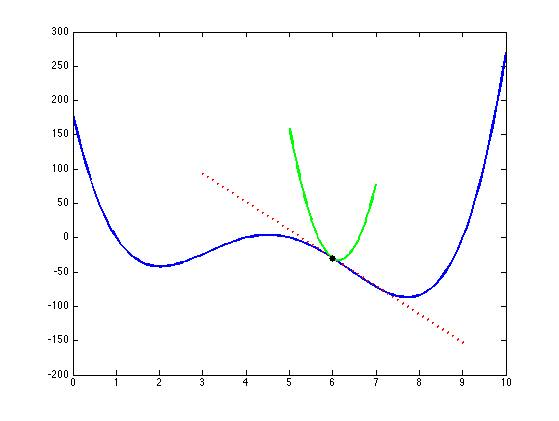
\includegraphics[scale=0.6]{./images/Course5_construction} 
\caption{In blue: $f$ of $C_L^{1,1}$, in red: tangent to the function, in green: the QUB}
\label{5:fig1}
\end{center}
\end{figure}

\begin{lemma}
\textbf{Quadratic upper bound (QUB) of $C_L^{1,1}$ function} \\
Let's $f \in C_L^{1,1}$. Then for any $x$ we have that 
$$ \hat{f}: y \mapsto  f(x)+ \nabla f^T(x)(y-x)+ \frac{L}{2} \| y-x\|^2_2 $$
 is an upper bound of $f(y)$.
\end{lemma}

Notice that $\hat{f}$ is a quadratic function of $y$.  What is the minimum of the quadratic upper bound? Our function is now convex and easy to minimize over $y$.


$$\nabla \hat{f}(y)=0 \Leftrightarrow  \nabla f(x) +\frac{L}{2} 2(y-x)=0$$

$$ \Rightarrow y^{*} = x- \frac{1}{L} \nabla f(x)$$

We can notice that the last equation is very similar to the gradient method. It is sensible to use $h_k=\frac{1}{L}$ in our method. 

\subsection{Analysis of the $h_{k}$= $\frac{1}{L}$ gradient method}
 
After one step, taking  $y= x-\frac{1}{L}\nabla f(x)$, the upper bound gives:
\begin{align*}
\hat{f}(y)=f(x) + \nabla f(x)^{T} [\frac{-1}{L} \nabla f(x)]+\frac{L}{2} \|  \frac{-1}{L}\nabla f(x)\|^2
& =f(x)- \frac{\|\nabla f(x)\|^{2}}{L}+\frac{1}{2L} \|\nabla f(x)\|^{2} \\
& =f(x)-\underbrace{\frac{1}{2L} \|\nabla f(x)\|^{2}}_{\leq 0}
\end{align*}
Looking at all iterations now:
$$ f(x_{k+1})-f(x_{k}) \leq - \frac{\|\nabla f(x_k)\|^{2}}{2L}$$
(because the upper bound displays this decrease \textcolor{red}{What does it mean?})\\


$f(x_1)-f(x_0) \leq -\dfrac{\|\nabla f(x_{0})\|^{2}}{2L}$\\
$f(x_2)-f(x_1) \leq -\dfrac{\|\nabla f(x_{1})\|^{2}}{2L}$ \\
$\vdots$ \\
$f(x_{N+1})-f(x_N) \leq -\dfrac{\|\nabla f(x_{N})\|^{2}}{2L}$\\

Summing the equations above, we get \\
$f(x_{N+1})-f(x_0) \leq - \dfrac{1}{L} \sum\limits_{i=0}^{N}$ $\|\nabla f(x_{i})\|^{2}$\\
so we deduce \\
$2L(f(0)-f(N+1)) \geq \sum\limits_{i=0}^{N} \|\nabla f(x_{i})\|^{2} \geq (N+1) \min \|\nabla f(x_{i})\|^{2}$

Hence
\begin{align*}
\underset{i=0,...,N}{\text{min }} \|\nabla f(x_{i})\| & \leq \sqrt{\frac{2L(f(0)-f(N+1))}{N+1}} \\
& \leq \sqrt{\frac{2L(f(0)-f(x^*))}{N+1}}
\end{align*}
with $x^*$ minimum point of $f$.
 
\begin{example}\begin{leftbar} Behaviour of the gradient method
$$2x^{2}+y^{4}-2y^{2}$$
we start from (1,0)

 \begin{equation*}
   \nabla=
 \begin{pmatrix}
4x  \\
4y^{3}-4y
\end{pmatrix}
\end{equation*}

\begin{equation*}
   \nabla^{2}=
 \begin{pmatrix}
4 & 0 \\
0 & 12y^{2}-4
\end{pmatrix}
\end{equation*}
We have three stationary points $(0,0)$,$(0,1)$,$(0,-1)$. 

We observe that
 \begin{equation*}
   \nabla(1,0)=
 \begin{pmatrix}
4  \\
0
\end{pmatrix}
\end{equation*}
If we start from $(1,0)$, we can only converge to $(0,0)$ (which is a saddle point) and we couldn't find all the points. 
\end{leftbar}\end{example}








%\end{document}
